\documentclass{article}
\usepackage[UTF8]{ctex}
\usepackage{amsmath}
\usepackage{fancyhdr}
\usepackage{geometry}
\usepackage{pgf-pie}
\usepackage{sectsty}
\usepackage{xcolor}

\geometry{left=3cm, right=3cm, top=3cm, bottom=3cm}

\title{6G技术调查报告}
\author{Koorye}
\date{2024年3月5日}

\pagestyle{fancy}
\fancyhead[L]{移动计算技术——第一次作业}
\fancyhead[R]{Koorye}
\fancyfoot[R]{基于\LaTeX 排版制作}

\begin{document}
\maketitle
\thispagestyle{fancy}

\section{国内外研究与应用现状}

\begin{figure}[h]
\centering
\begin{tikzpicture}
    \pie[cloud]{35/中国, 18/美国, 13/欧洲, 13/日本, 10/韩国, 11/其他}
\end{tikzpicture}
\caption{各国6G技术专利申请概况}
\label{fig:6g-submit}
\end{figure}

6G技术\cite{jiang2021road}是指第六代移动通信技术,是5G技术的升级版。国内外的6G技术都在不断的发展。在国内,中国的政府机构、运营商、通信企业等都在积极的推进6G技术;在国外,美国、日本、韩国等国家也在积极的推进6G技术的研究和应用。与先前通信技术相比,6G技术的目标是提供更高的数据传输速率、更低的延迟、更高的可靠性、更低的能耗、更大的连接密度、更广的覆盖范围等。6G技术将为将为虚拟现实、增强现实等新型应用提供更加优化的条件。

国内的6G技术正在被积极的推进。中国信通院的IMT-2030(6G)推进组发布了《6G总体愿景与潜在关键技术》白皮书,涵盖了6G的总体愿景、八大业务应用场景和十大潜在关键技术,包括实现智能化、高效互联,从万物互联到万物智联,为人类社会可持续发展做出贡献。同时,华为也发布了名为《6G:无线通信新征程》的白皮书,提出6G将跨越5G,从服务于人、人与物,进一步拓展到支撑智能体的高效互联,实现万物智联的跃迁。总之,国内对6G技术的研究和应用正处于积极探索和发展的阶段,各界都对其前景寄予厚望。

而在国外,6G技术同样备受关注。美国、欧盟、日本等国家和地区都在积极的推进6G技术的研究和应用。美国众议院去年年底通过了旨在加强6G通信技术竞争力的《未来网络法案》,旨在美国联邦通讯委员会(FCC)组成“6G特别工作小组”,开发6G技术。此外,美国民间企业结成next G联盟,正式展开确保6G标准技术处于市场领先地位的活动。而欧盟正在以2030年建立6G生态系统及商用化为目标进行大规模投资,成立了民间企业6G研究开发集团“HEXA X”,该集团将研究开发6G核心技术人工智能(AI)基础技术、扩大服务覆盖范围、网络可持续性技术等。此外,日本还将以加强6G全球竞争力为目标,推行“Beyond 5G”推进战略。总的来说,各国对6G技术的研究和应用都十分重视,且都在积极的推进。

目前各国对6G技术展开激烈竞争,而中国在其中占用主导地位。如图\ref{fig:6g-submit}所示,中国国家知识产权局公布的《6G通信技术专利发展状况报告》显示,中国在6G技术专利申请数量上占据绝对优势,占比达35\%,远超美国的18\%,以及其他国家的占比。这次6G技术将会深化一些主要通信发达国家之间的标准化竞争,各国技术霸权战争愈演愈烈。在6G时代,全球标准开发很有可能会在比合作关系更密切的竞争体制下进行。

\section{采用的技术手段}

\begin{figure}[tb]
    \centering
    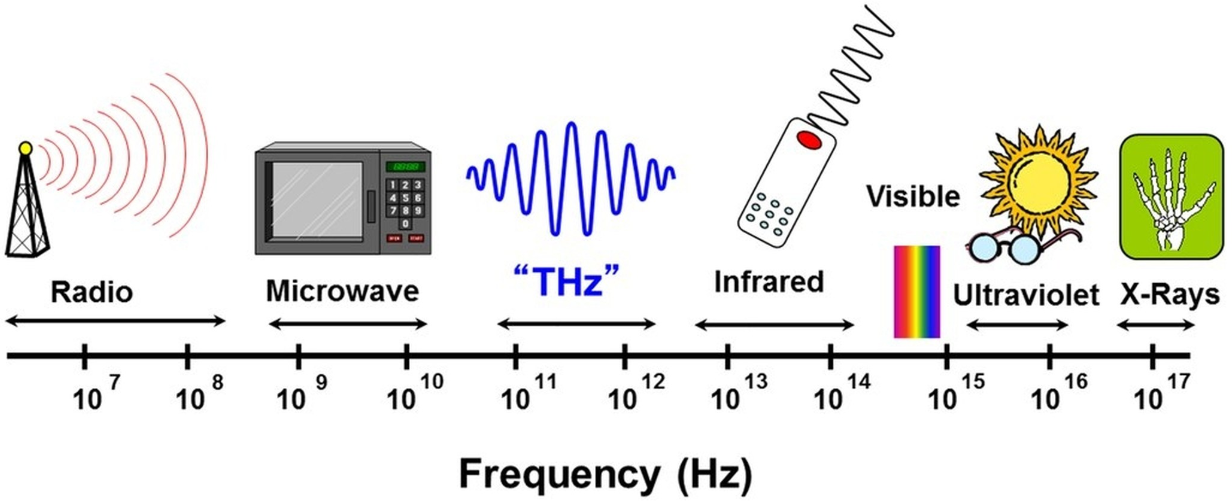
\includegraphics[width=\textwidth]{pics/太赫兹.png}
    \caption{太赫兹波段对比}
    \label{fig:thz}
\end{figure}

6G技术的研究和应用涉及到多个领域,包括通信技术、计算机技术、人工智能技术、物联网技术等。下面将介绍其中的一些关键的技术手段。

\textbf{太赫兹技术}\cite{siegel2003thz}。太赫兹技术是6G技术的关键技术之一。如图\ref{fig:thz}所示,太赫兹波段是指100GHz到10THz的频段,是微波和红外光之间的频段。太赫兹波段的频谱资源丰富,传输速率高,能够实现高速数据传输。太赫兹波同时具备了微波通信和光通信的优点,具有波束窄、方向性好的特点。同时,由于太赫兹波的波段较短,可以大大缩小终端天线的大小。总的来说,太赫兹技术将会大大提高数据传输速率,同时提升设备稳定性,为6G技术提供更加优化的条件。

\textbf{通信感知一体化(ISAC)技术}\cite{dilling2014isac}。通信感知一体化技术是6G技术的另一个关键技术。通信感知一体化技术是指将通信技术和感知技术相结合,使得一切业务、网络、用户和终端,以及环境物体的属性与状态的通信系统,其在感知的上可具有超出传统雷达的能力。通过让通信系统和感知系统共享资源、硬件等设施,两者可以协同完成波形设计、信号处理、协议接口、组网协作等复杂任务。通信感知一体化技术将会提高通信的可靠性和安全性,助力6G技术发展。

\textbf{智能超表面(RIS)技术}\cite{liu2021reconfigurable}。智能超表面,也叫做“可重配智能表面”,或者“智能反射表面”,能够定义新的无线传输和传播模式,并控制通信信道。智能超表面通过实时调整无源反射元件的吸收、反射、折射和相位,从而将入射电磁信号引导到所需方向,实现有效信道增益最大化。智能超表面技术将会提高通信的覆盖范围和传输速率,为6G技术提供技术支撑。

\section{发展方向和挑战}

6G技术作为第六代通信技术,将会在5G技术的基础上进一步提高数据传输速率、降低延迟、提高可靠性、降低能耗、提高连接密度、扩大覆盖范围等。6G技术的发展方向主要有以下几个方面。

\textbf{全域覆盖}。在空间上,6G技术将实现更广泛的覆盖,连接空中、地面和太空。在设备上,6G技术得覆盖对象将扩展到环境感知设备,连接环境与通信系统,实现智能化。

\textbf{高速传输}。6G技术将实现更高的数据传输速率,提高网络的容量和速率,实现更快的数据传输。

\textbf{跨界融合}。6G技术可能与其他信息技术深度融合,如人工智能、物联网、区块链等,实现更多的应用场景。

\textbf{数据本地化}。6G技术可能实现数据的本地化存储和处理,提高数据的安全性和隐私性。

\textbf{通信、感知和计算的结合}。6G技术可能提供连接、感知、算力的能力网络。利用无线感知主动获取数据,利用通用计算提供便捷性,6G系统可及时进行更新与迭代,提供更强大的通信与连接服务。

\textbf{协议开放}。6G技术可能会提供定制接口满足用户的多样化需求,或者以资源租借的方式向用户提供设备服务。

同时,6G技术的发展也面临着一些挑战。

\textbf{海量接入问题}。6G技术将会连接更多的设备,尽管 6G 网络可以使用更高的带宽,但是多个终端设备接入网络需要非常强壮的多址接入方法和更好的动态分配机制等,这也是目前很难做到的。海量接入问题将会成为一个挑战。

\textbf{节能供电问题}\cite{mao2021ai}。不仅通信网络会持续造成能源消耗,另外人工智能的算力应用广泛,计算复杂度很高,能耗极大。6G技术需要在节能供电方面做出更多的努力。

\textbf{实时性问题}\cite{cao2020delay}。6G技术将会覆盖天空和海洋,同时要满足随时随地的连接和通信需求,这将会对6G技术的实时性提出更高的要求。

\textbf{网络安全问题}\cite{nguyen2021security}。6G技术将会产生前所未有的大量隐私数据,如何保障个人隐私数据安全,将会是一个重大挑战。

\textbf{非技术性问题}。一些非技术性壁垒,如资金、政策,国家间的协议和标准等,也将会对6G技术的发展产生影响。

\section{6G的应用场景}

6G技术涉及通信、感知和计算领域,具有丰富的应用场景。其中的一个典型应用是自动驾驶领域\cite{chen2020deep,yang2021edge}。自动驾驶技术需要实时获取车辆周围的环境信息,包括道路、车辆、行人等,同时需要实时的传输数据,以及实时的决策和控制,恰好对应6G技术中的感知、通信和计算3个部分。因此,自动驾驶对环境感知的准确性、通信的实时性、计算的高效性等方面提出了更高的要求。下面将介绍自动驾驶领域的特殊要求,以及基于6G技术的解决方案。

\textbf{高精度感知}。自动驾驶需要实时获取车辆的位置信息,以及周围环境的地图信息,如行人、障碍物等。6G技术通过物联网技术,检测道路车辆周围的环境,实现高精度的定位。

\textbf{高速数据传输}。自动驾驶对周边环境的实时性要求极高,在高速行驶的情形下,如果车辆前方突然出现障碍物,需要实时的传输数据,以及实时的决策和控制。6G技术通过太赫兹技术,实现高速的数据传输,以及低延迟的通信。

\textbf{快速决策}。自动驾驶需要实时的决策和控制,依赖高效的计算。一种方案是各个车辆通过各自的设备独立进行运算,然而这样会造成大量的重复计算,浪费资源。6G技术通过庞大的通信网络,实现车辆之间的通信和协作,共享资源、硬件等设施,实现高效的计算以作出决策。

基于6G技术,自动驾驶领域将会实现更高的精度、更快的速度、更高的安全性,为人类社会带来更多的便利。

\bibliographystyle{plain}
\bibliography{ref}

\end{document}